\chapter{Embedded System for Online Fault Detection and Diagnosis}

Having evaluated the CML at nCATS, and the ability of cheap sensors and hardware to classify conditions, an embedded CMS is presented.
The design is discussed, including the philosophy behind the software design.
A long term test is performed, attempting to create more realistic conditions.
The energy use of the final system is measured and inspected.

\section{System Design}

\subsection{Hardware}

The embedded CMS includes elements of MCSA and vibration analysis.
Therefore, it uses CTs and MEMS sensors.
For the purposes of this project, one sensor of each is used, although more could be added in the future for a more complex machine or more complex analysis.
The test setup and hardware of the system is shown in Fig \ref{fig:SystemHardware}.
It combines the setup of separate tests which were performed in the previous chapter.
Additionally, to emulate an industrial system and increase the safety of the system, the CT has been soldered to long wires and the connections insulated with heat shrink (Fig \ref{fig:HeatShrink}).
This allows the CT to sit inside the motor control box, which is connected to high power lines.
The CT wires travel safely from the box to the MSP432 which sits inside the CML casing.
In a working environment, such as on board a ship, there are strict electrical standards which wiring must adhere to \cite{BS7917-1999}.
To prevent noise from interfering with signals, shielded and twisted core cables should be used.
Communication and power is provided by a USB cable which extends into the casing.
This means that the system can be fully operated remotely.
The safety of testing is improved and requirements of the system more realistic.
\par

\begin{figure}
    \centering
    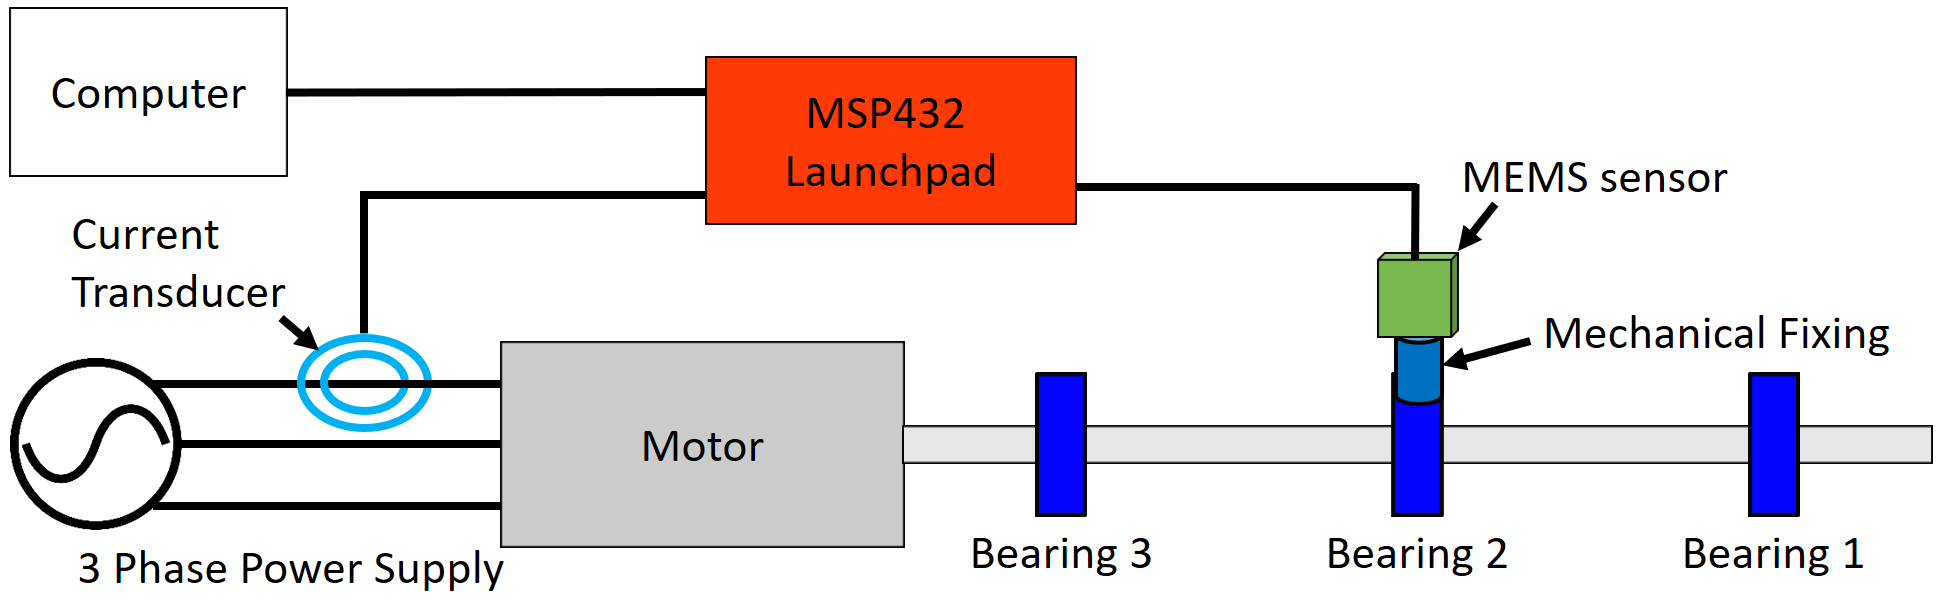
\includegraphics[width=\linewidth]{SystemHardware.PNG}
    \caption{Diagram of embedded CMS setup for test on the CML at nCATS}
    \label{fig:SystemHardware}
\end{figure}

\begin{figure}
    \centering
    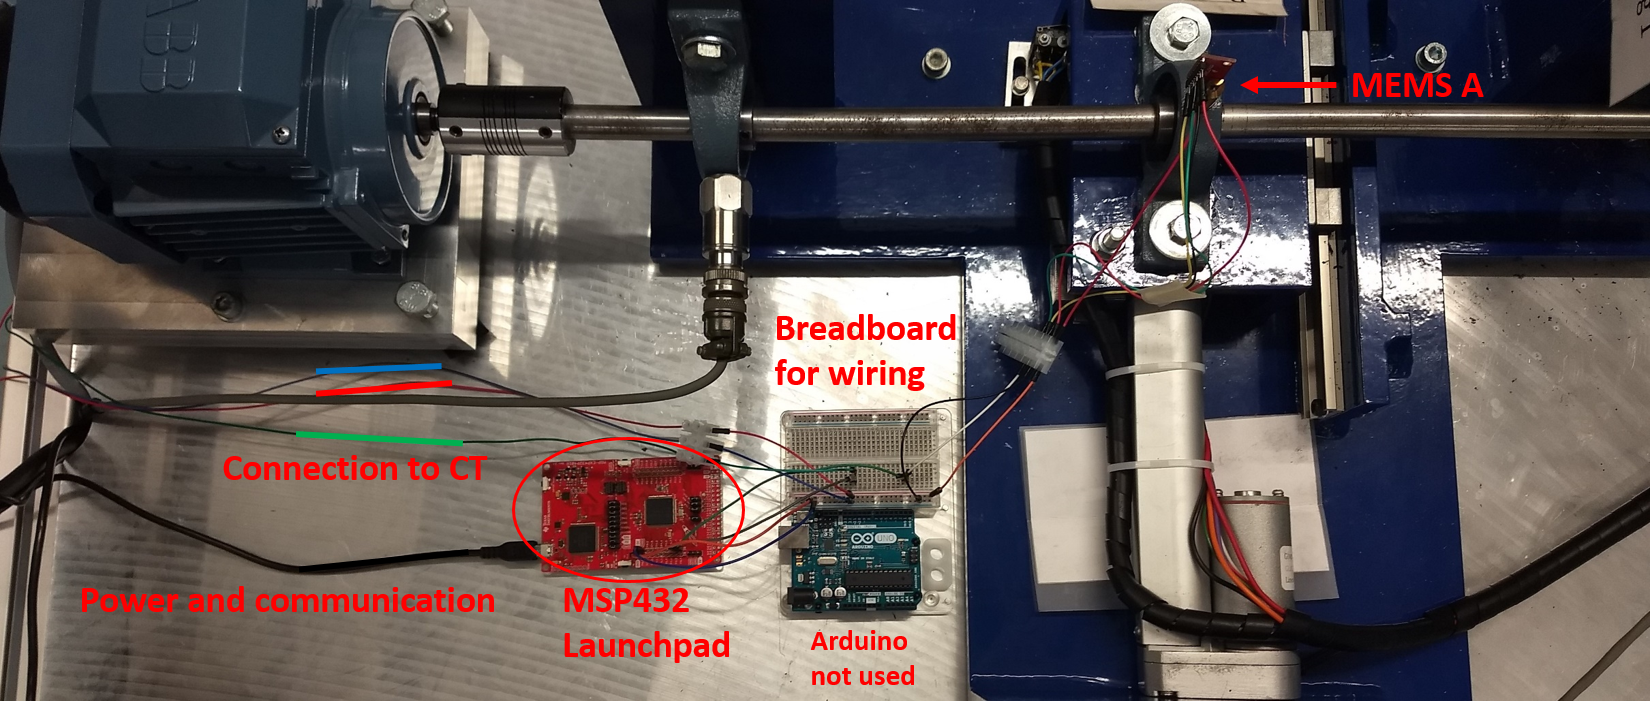
\includegraphics[width=\linewidth]{Images/EmbeddedCMS_Notes.png}
    \caption{Photo of test setup on the CML at nCATS}
    \label{fig:EmbeddedCMS}
\end{figure}

\begin{figure}
  \centering
  \begin{subfigure}[b]{0.3\linewidth}
    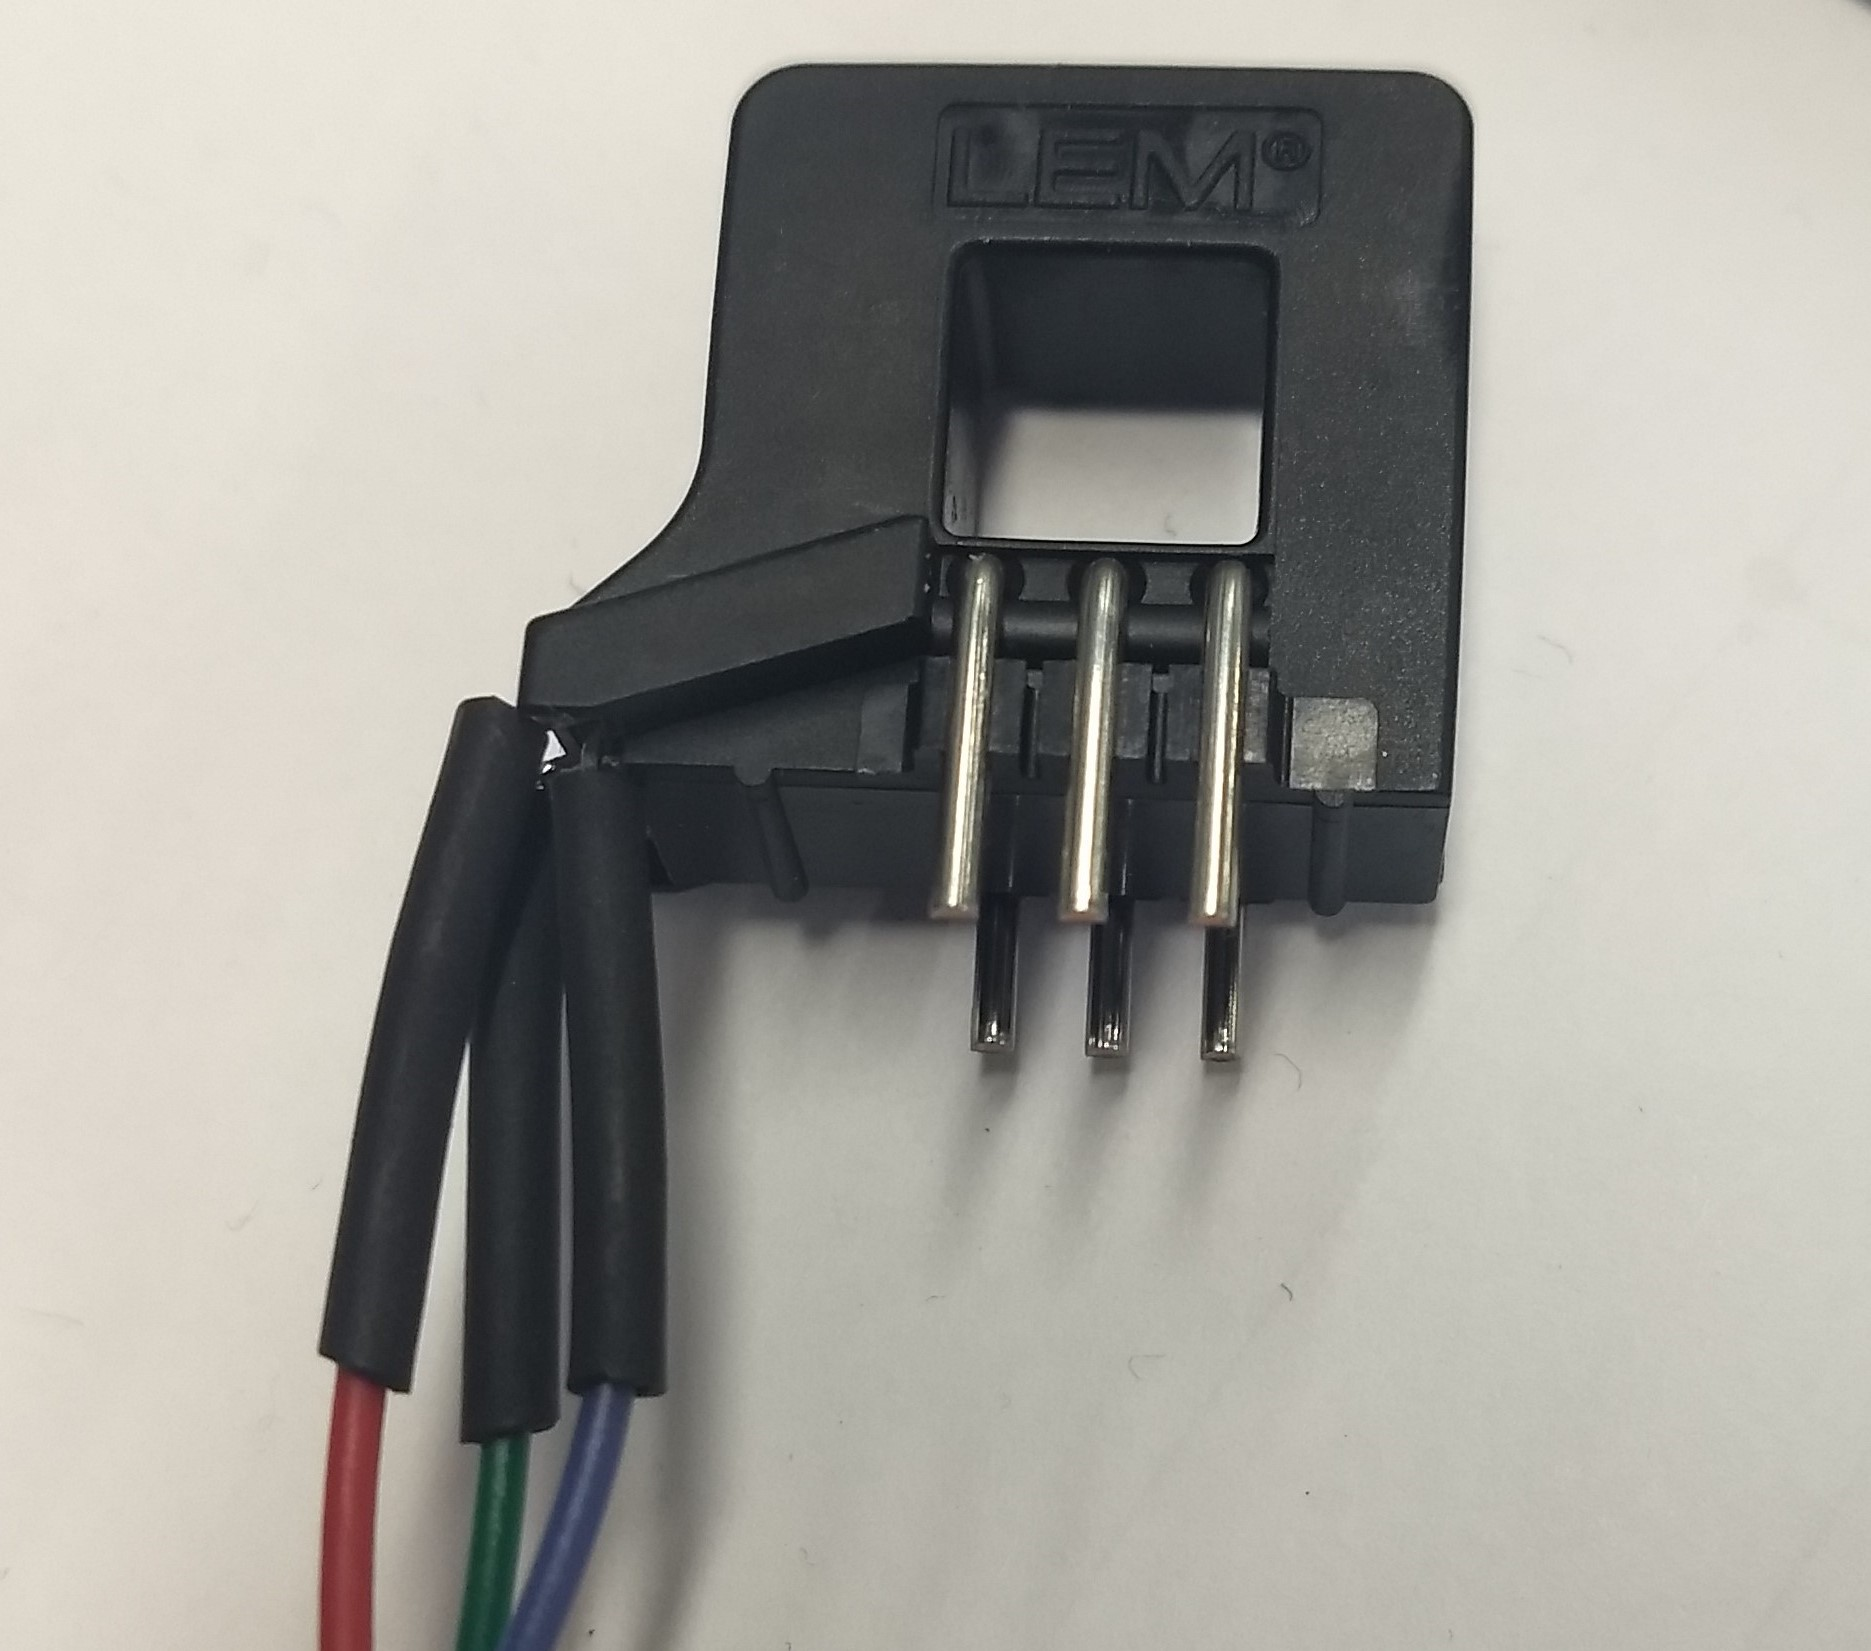
\includegraphics[width=\linewidth]{Images/Current_Sensor.jpg}
    \caption{Heat shrink on CT connections}
  \end{subfigure}
  \begin{subfigure}[b]{0.3\linewidth}
    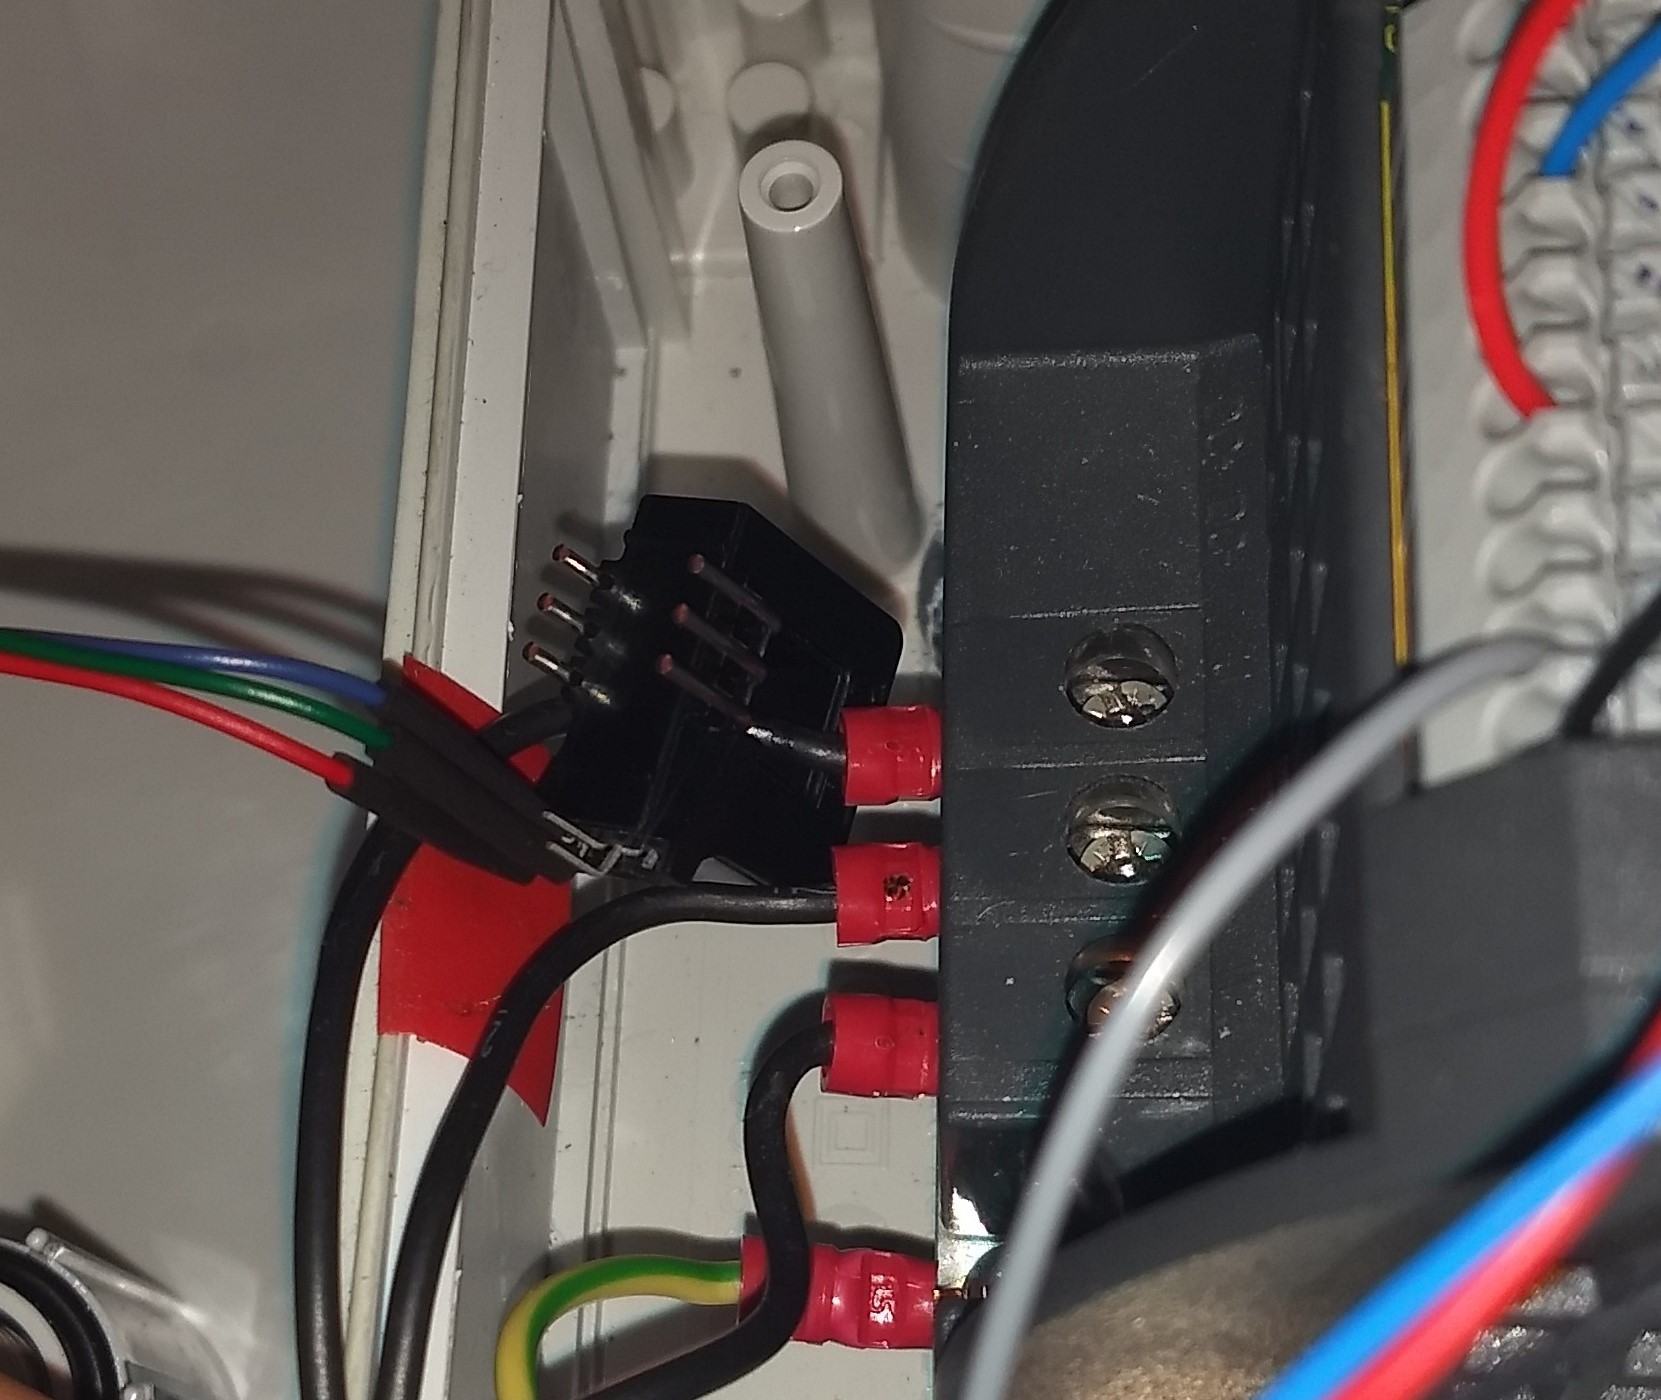
\includegraphics[width=\linewidth]{Images/CT_Box.jpg}
    \caption{CT mounted inside motor control box}
  \end{subfigure}
  \begin{subfigure}[b]{0.3\linewidth}
    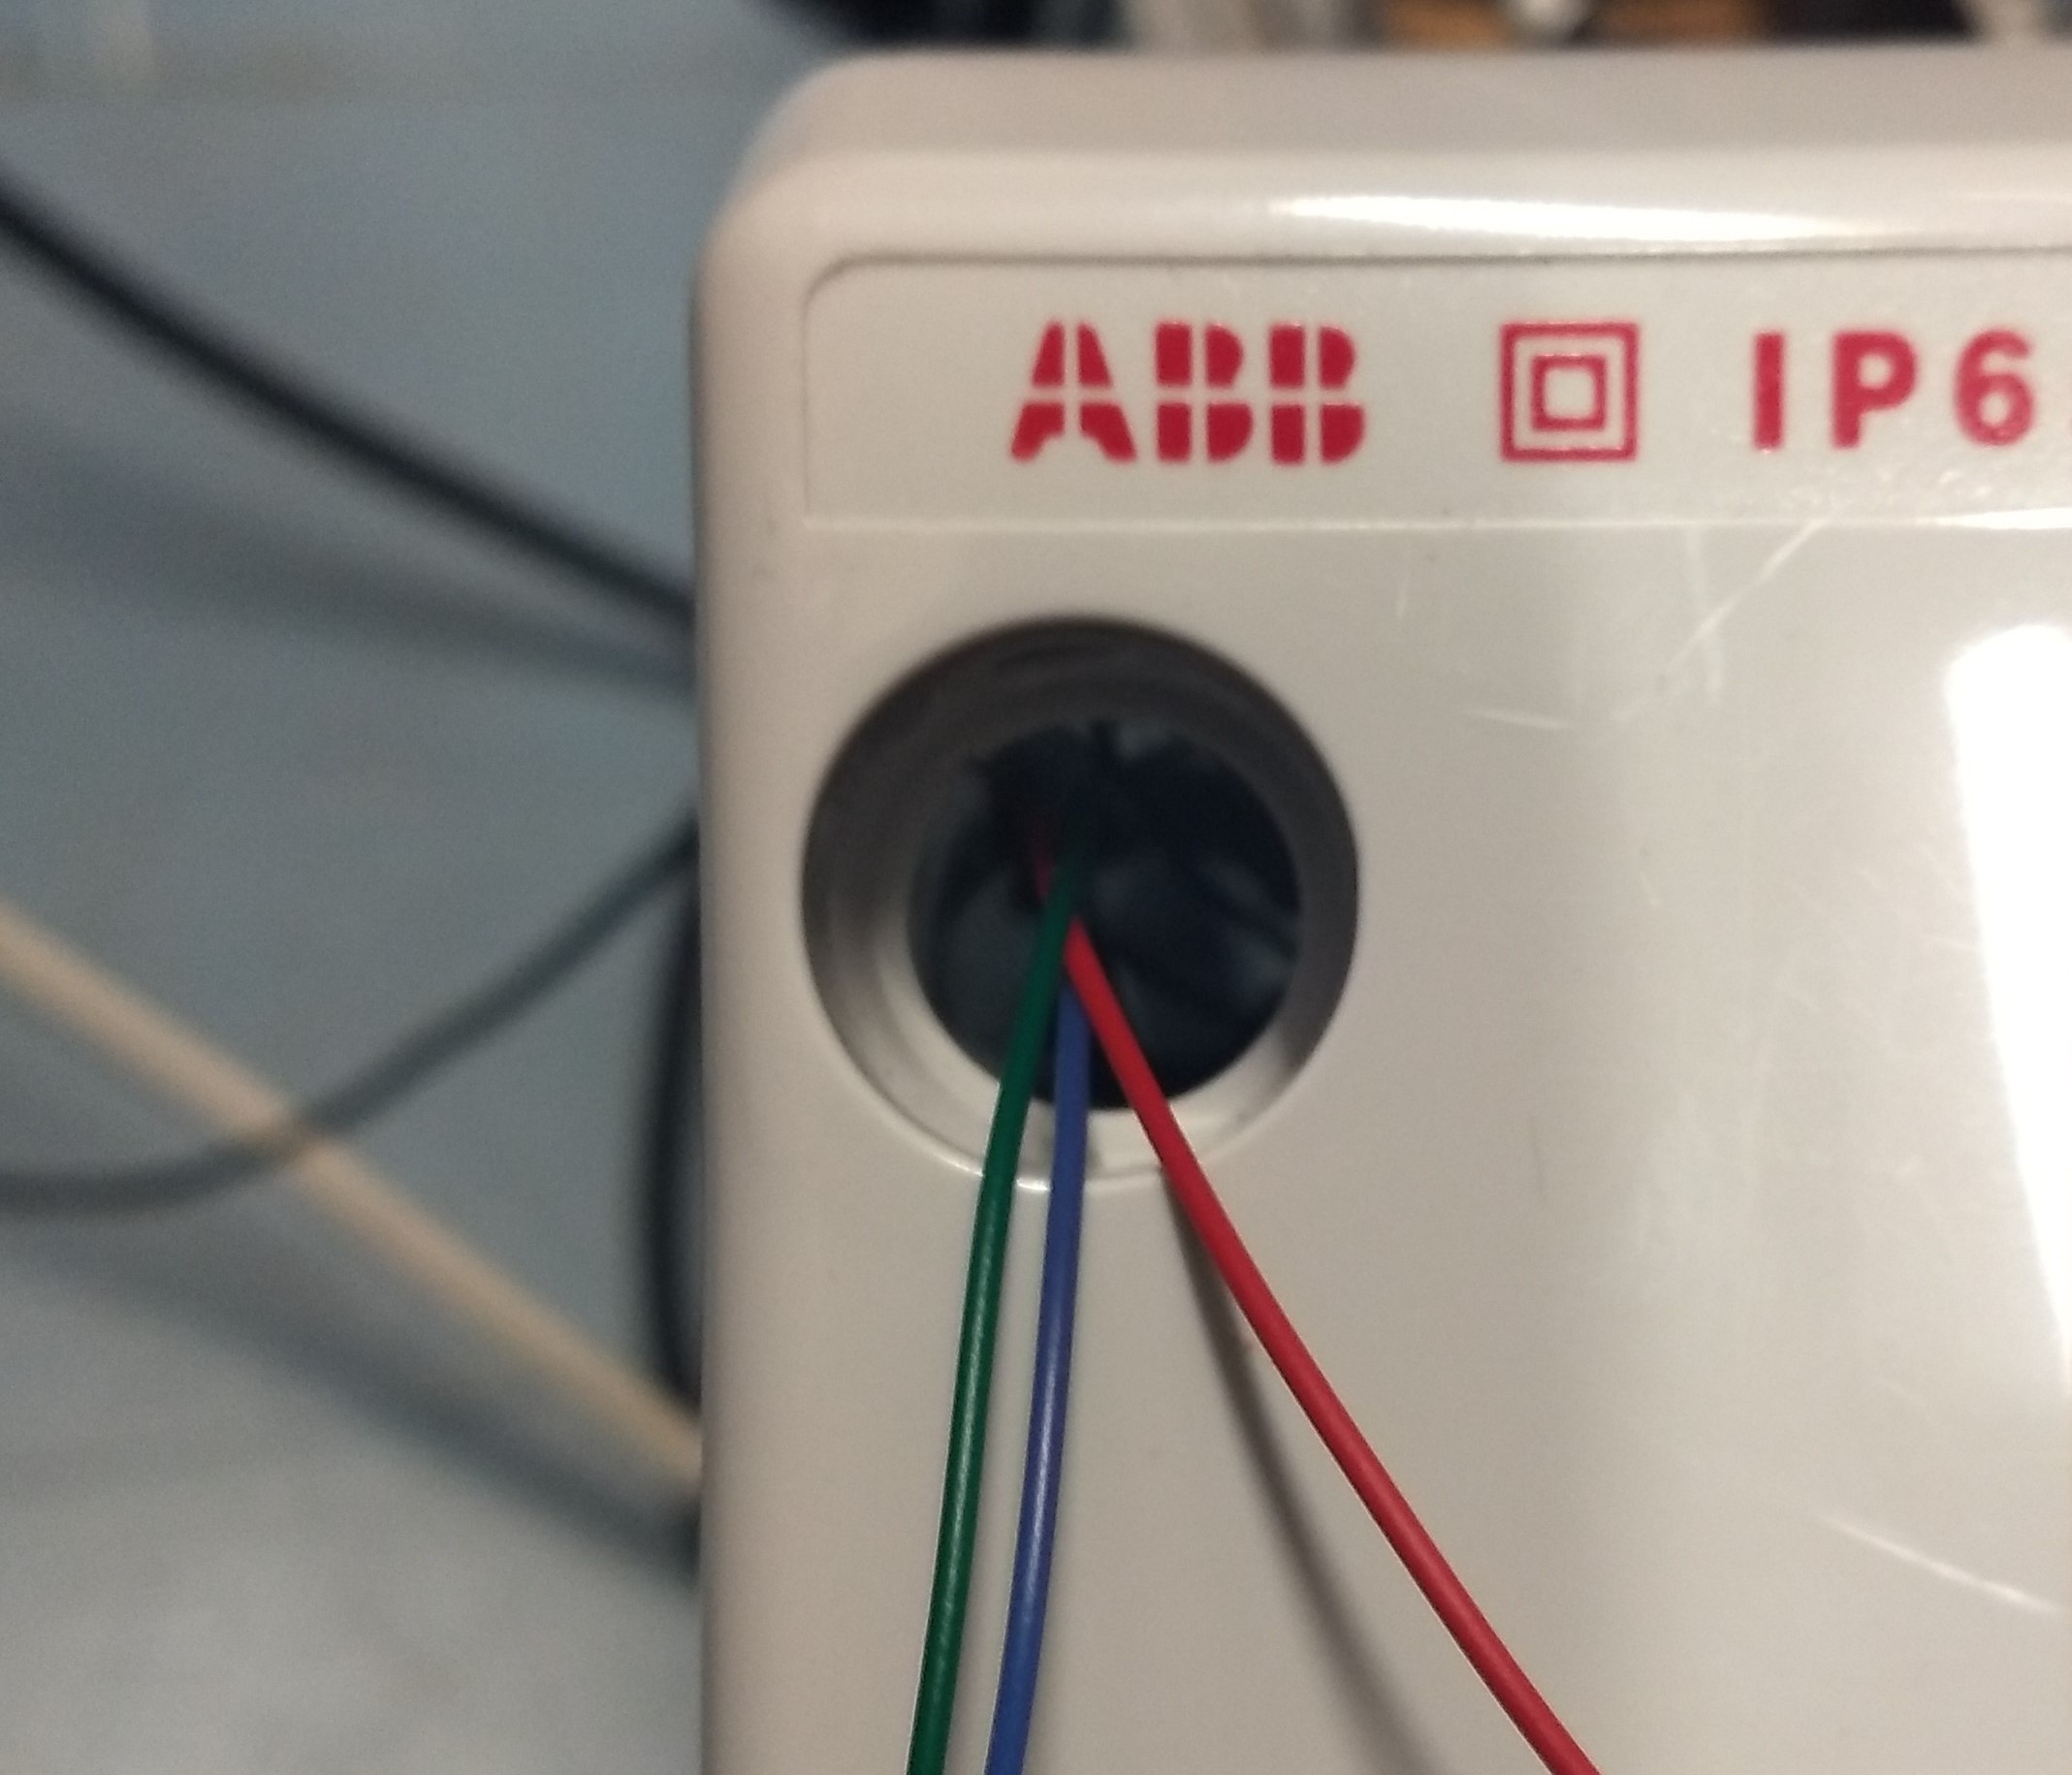
\includegraphics[width=\linewidth]{Images/CT_Box2.jpg}
    \caption{Wires connected safely to CT}
  \end{subfigure}
  \caption{CT setup for testing of embedded CMS}
  \label{fig:HeatShrink}
\end{figure}

\subsection{Software}

The software for the system follows the flow chart laid out in Fig \ref{fig:SW_Flowchart}.
Interrupts are used to trigger readings and capture ADC data.
Read triggers are:
\begin{itemize}
    \item \textbf{Real-Time Clock (RTC)} - Triggers a reading once every minute
    \item \textbf{Serial Interface} - Triggers a reading upon reception of a certain message
    \item \textbf{Push Button} - Useful for sanity checks
\end{itemize}

Once a new reading is triggered, the current sensor is sampled first at 4096 Hz.
If the motor is found to be running at full speed - the condition which has condition information - then vibration readings are also triggered.
A message containing MCSA information is sent to the computer.
\par

If vibration readings are triggered, the accelerometer is read at 8192 Hz.
Both the time domain and frequency domain are inspected and decisions about condition are made.
If an instruction to set a new healthy state has been detected, this information is recorded.
Messages with vibration analysis information are sent to the computer.
\par

While this information could be processed by a central node to provide diagnosis, all processing and decisions are performed on-board.


\begin{figure}
    \centering
    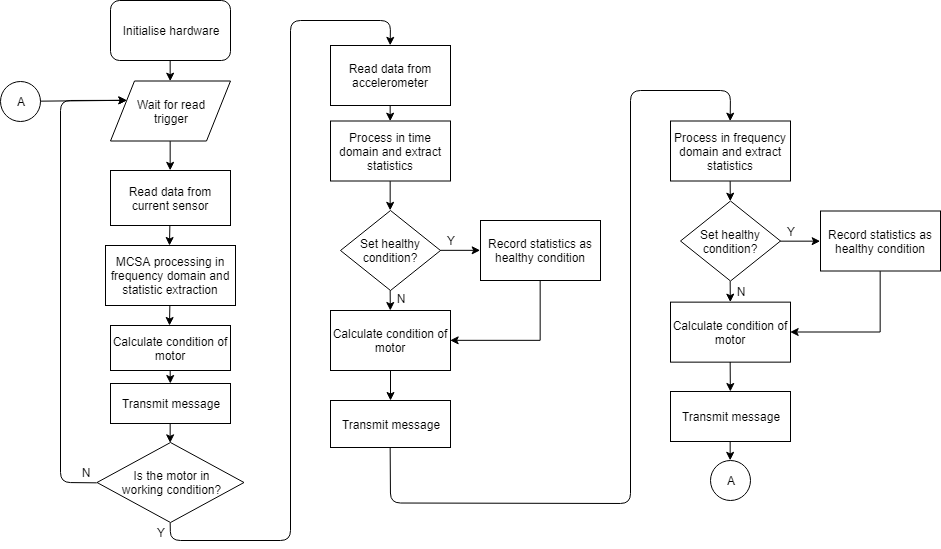
\includegraphics[width=\linewidth]{software1.png}
    \caption{Software flow chart for embedded CMS}
    \label{fig:SW_Flowchart}
\end{figure}

\subsection{Decision Making}

The main output of interest from the embedded CMS is the current condition of the rig.
The algorithm for this classification is basic but based on the information generated from testing the sensors on the rig.
\par

The CT is primarily used to identify the rotor speed.
The maximum of the frequency spectrum is identified.
If it is found to be below approximately 0.04 A, the motor is identified as being stopped, as the main component is far below the magnitude expected from a running motor.
If the maximum is above this level, the maximum frequency is used to identify the state of the motor.
Between 48 and 52 Hz, the motor is identified as running, giving some allowance for error in measurements or calculation.
Below that, the motor is identified as in a loading state.
It is expected that at those frequencies, the motor is either starting up or stopping.
Above 52 Hz is unexpected behaviour and the motor is identified as unhealthy.
\par

Vibration analysis is used in both the time and frequency domain.
The classifications are made with respect to `Healthy' values which are set during operation.
`Healthy' values create a baseline against which changes can be measured.
Limits are made relative to this baseline based on the tests covered in the previous chapter.\\
In the time domain, conditions are:
\begin{itemize}
    \item \textbf{Healthy} - $0.8*RMS_{healthy} < RMS < 1.2*RMS_{healthy}$ and $max < 1.5*max_{healthy}$
    \item \textbf{Bearing Fault} - $0.8*RMS_{healthy} < RMS < 1.2*RMS_{healthy}$ and $max > 1.5*max_{healthy}$
    \item \textbf{Unhealthy} - Else
\end{itemize}
In the frequency domain:
\begin{itemize}
    \item \textbf{Healthy} - $0.8*max_{healthy} < max < 1.2*max_{healthy}$
    \item \textbf{Bending} - $max < 0.5*RMS_{healthy}$ and $std < std_{healthy}$
    \item \textbf{Unhealthy} - Else
\end{itemize}

These classifications are shown relative to the average values of the samples tested in the previous chapter in Fig \ref{fig:Condition_Decision}.
While the limits are basic, they should prove effective.
As the healthy state of the CML is known to change, making decisions relative to a set state allows for proper testing to take place, as opposed to strict numerical limits.
Monitoring changes in signal has also been found to be a sensible approach for a range of machinery \cite{CM_randall}.

\begin{figure}
    \centering
    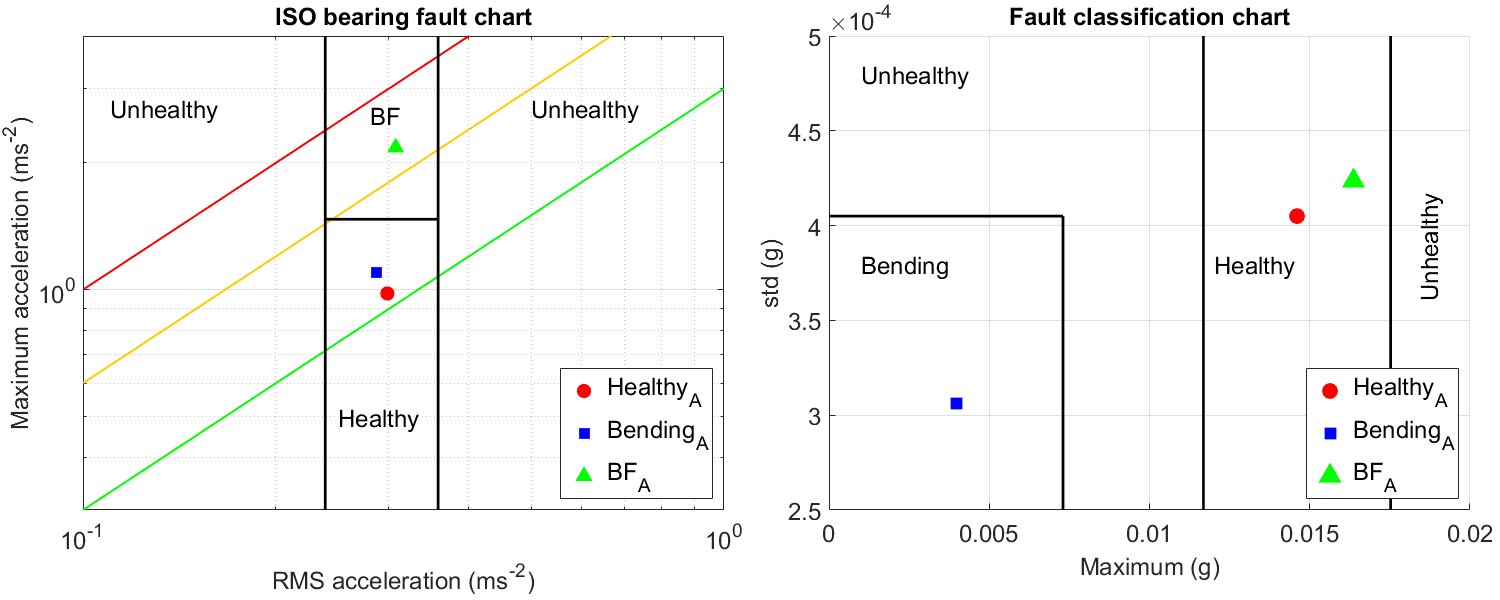
\includegraphics[width=\linewidth]{Condition_Decision.png}
    \caption{Charts showing how condition is diagnosed using time domain (bearing fault severity) and frequency domain (fault classification)}
    \label{fig:Condition_Decision}
\end{figure}

\subsection{Communication}

There are many protocols and methods for communication of condition monitoring systems \cite{Embedded_Comms}.
The embedded CMS uses serial communication combined with NMEA 0183, a popular protocol for GPS units and other devices in the maritime industry \cite{NMEA_website}.
It is a simple protocol, which is also easy to implement, and relevant to the future application of this system.
An industrial implementation would have to meet wiring standards for RS232, but for testing the message is sent over a USB cable at low voltage \cite{NMEA_website}
The data fields and expected values are detailed in Table \ref{tab:NMEA_format}.
The messages are read and stored on the computer using an NMEA Python library to interpret \cite{PythonNmea2}.
A custom class was created for the embedded CMS.


\begin{table}
    \renewcommand{\arraystretch}{1.5}
	\begin{center}
		\begin{tabularx}{\textwidth}{>{\hsize=.5\hsize}X>{\hsize=1\hsize}X}%Changed c to S
			\toprule
			\multicolumn{2}{c}{\$PCBM,...$<$0D$><$0A$>$}\\
			\cmidrule{1-2}
			\textbf{Data field} & \textbf{Notes} \\
			\midrule
			Identifier & \makecell[tl]{P - Proprietary message format \\ CBM - Sentence Type}\\
			Message type & \makecell[tl]{M - MCSA \\ V - Vibration Analysis}\\
			Domain & \makecell[tl]{T - Time domain \\ F - Frequency Domain}\\
			Hour & Hours since start (0-99)\\
			Minutes & Minutes past hour (0-60)\\
			Max Freq & Frequency with largest component\\
			Maximum & Magnitude of largest value (0-65535)\\
			RMS & RMS of values in domain (0-65535)\\
			Std & Standard deviation of values in domain (0-65535)\\
			Condition & \makecell[tl]{MCSA:\\ R - Running \quad S - Stopped\\ L - Loading up/down \quad U - Unhealthy\\ Vibration analysis:\\H - Healthy \quad U - Unhealthy\\ B - Bending \quad F - Faulty Bearing}\\
			Runtime & Recorded runtime of motor\\
			\bottomrule
		\end{tabularx}
		\caption{Proprietary NMEA message format for ECMS}
		\label{tab:NMEA_format}%Can be referenced by rest of document
	\end{center}
\end{table}

\section{Long Term Test}

\begin{figure}
  \centering
  \begin{subfigure}[b]{0.4\linewidth}
    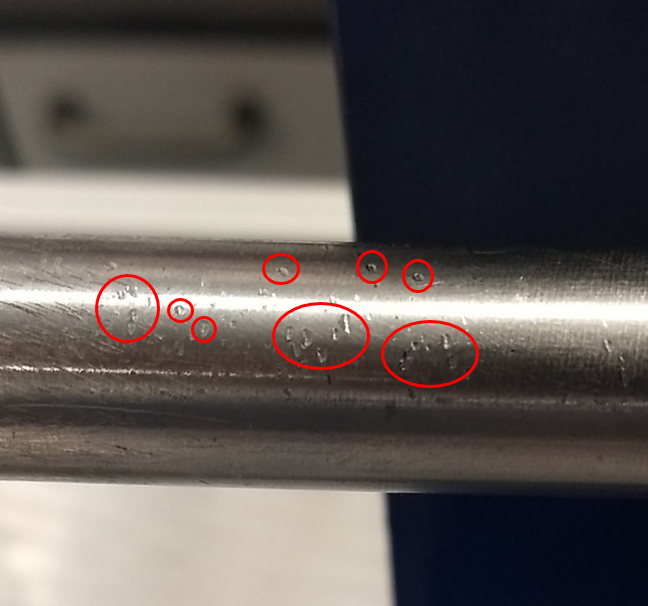
\includegraphics[width=\linewidth]{Damage1_Notes.png}
    \caption{Pock marks on shaft}
  \end{subfigure}
  \hspace{0.1\textwidth}
  \begin{subfigure}[b]{0.36\linewidth}
    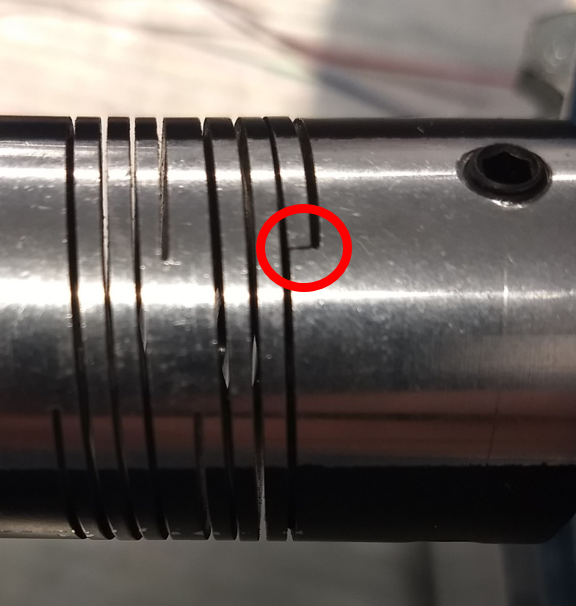
\includegraphics[width=\linewidth]{Damag2_Notes.png}
    \caption{Crack on flexible coupling}
  \end{subfigure}
  \caption{Damage on CML}
  \label{fig:Damage}
\end{figure}

To test the system adequately, it was necessary to run the CML for several hours continuously, varying the condition where possible while monitoring output from the system.
This would demonstrate the ability of the system to run independently and allow evaluation of the system accuracy in diagnosis.
Unfortunately, this precludes testing for a bearing fault, as changing a bearing on the CML is an arduous process and it is difficult to ensure that there are no other changes to the CML such as bending or movement.
While changing out the bearing during previous testing, damage was also made to the shaft and flexible coupling which could interfere with testing (Fig \ref{fig:Damage}).
Therefore, the test will induce healthy and bending states only.
Once a healthy state is stored, bending can be induced and should have a similar effect to the changes measured previously.
The motor will also be run up to and down from its full operating speed, to test the ability of the MCSA to identify the rotor speed.

\subsubsection{Results}



The output from the embedded CMS is displayed visually in Fig \ref{fig:LongTest_Overview}.
The system worked as expected, providing data every minute for four hours and setting new healthy states when requested.
MCSA effectiveness in identifying full running speed can be seen by the gaps in data for the vibration time and frequency domains, relative to the current level.
Differences between gradual motor run up/down and immediate starts/stops can also be seen on the MCSA chart where the current level is not stable and is identified as loading.
In this case, the current threshold proved effective, although in practice the background noise level may be higher and will have to be taken into account.
MCSA does not identify unhealthy behaviour in the motor, as expected.
\par



Within the time domain, only healthy and unhealthy conditions are transmitted.
This is expected as the faulty bearing was not tested for explicitly.
However, using the values from the time domain, the CML actually breaches the alarm limits for each vibration reading which was taken (Fig \ref{fig:LongTest_ISO}).
This suggests that there is in fact a significant fault with the CML in its current state.
It is possible that one of the bearings was damaged while preparing the CML for testing, although this would require further testing.
Future implementations could include numerical limits as a condition indicator.
There is significant variation shown for the max values, which is an effect of impulses caused by a fault.
When an unhealthy condition is identified it is often due to changes in the RMS value.
\par

The frequency domain, as expected, provides more information about the condition of the CML and is able to identify bending in several instances.
At times, bending was misdiagnosed as simply unhealthy.
The unhealthy diagnoses often align with unhealthy diagnosis from the time domain.
This suggests that faults other than simply bending may be surfacing.
Regardless of the exact cause, the system correctly identifies changes in condition.
The FFT max varies significantly across time and appears to be the prime indicator of condition.

\begin{figure}
    \centering
    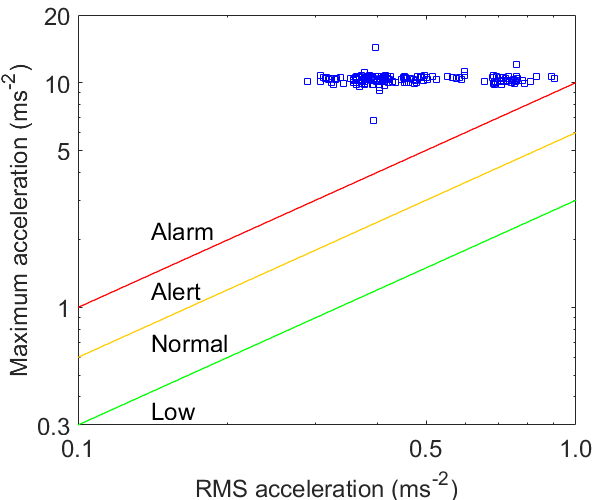
\includegraphics[width=0.7\linewidth]{LongTest_ISO_Bearing.png}
    \caption{Results from long term test time domain compared to ISO bearing fault standard}
    \label{fig:LongTest_ISO}
\end{figure}

\begin{landscape}
 \begin{figure}
  \centering
  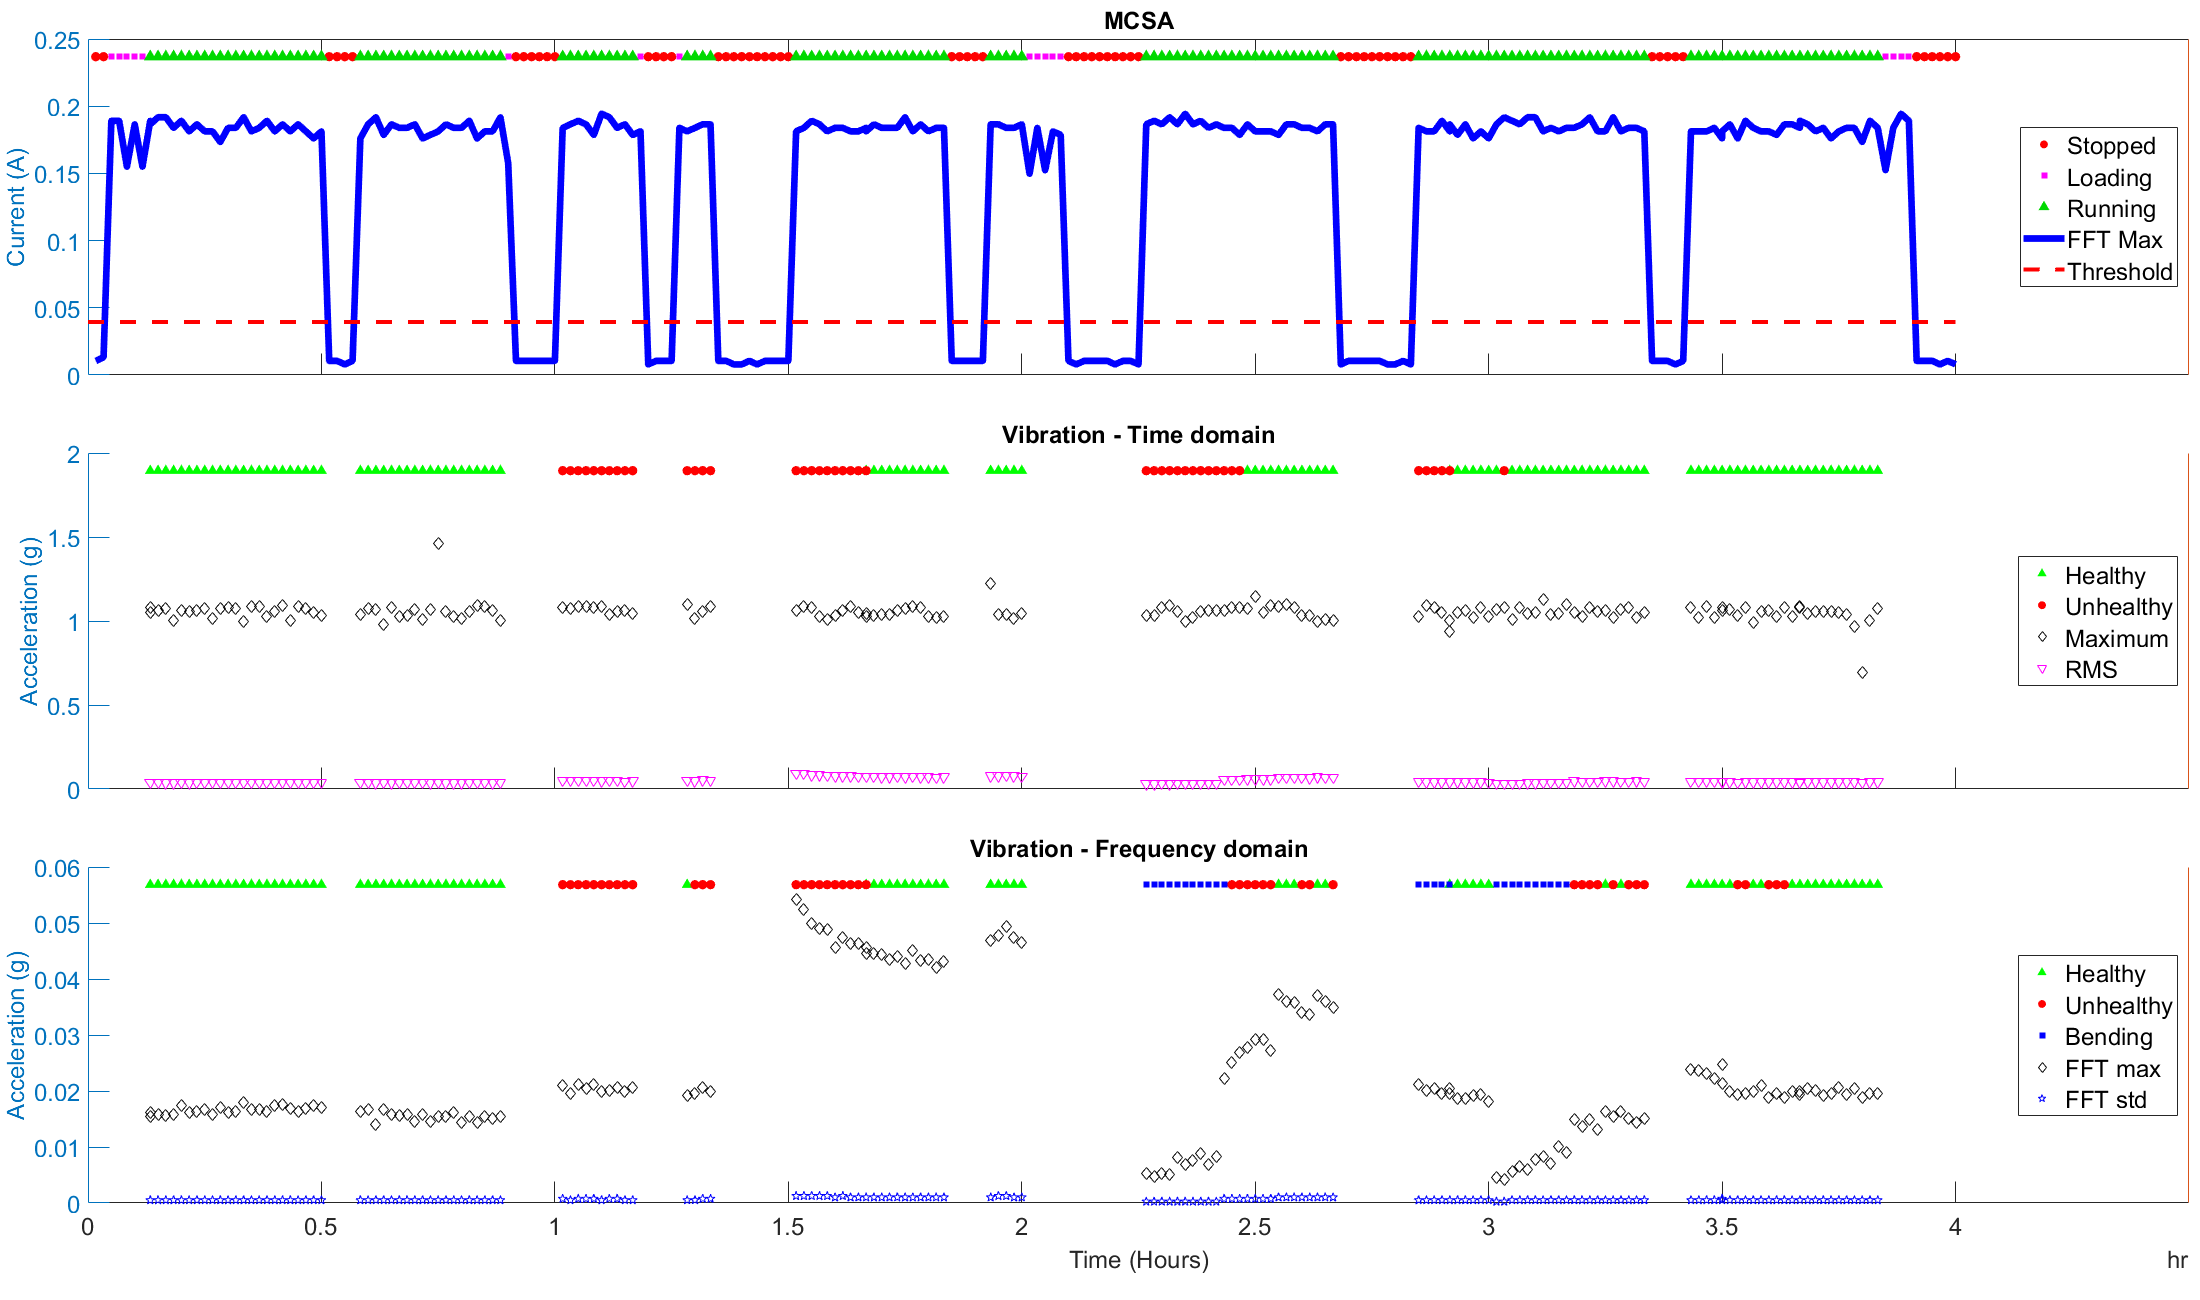
\includegraphics[width=\linewidth]{LongTest_Overview.png}
  \caption{Overview of results from long term testing of ECMS}
  \label{fig:LongTest_Overview}
 \end{figure}
\end{landscape}

\section{Power Consumption}

To inform further design decisions about the embedded CMS, power consumption of the system was monitored in several states.
The MSP432 Launchpad includes hardware specifically for monitoring power consumption as a program runs, through a technology known as EnergyTrace \cite{EnergyTrace}.
Energy consumption which travels through an on-board DC-DC converter is closely monitored, allowing even short device activity to be discerned.
The EnergyTrace tool in Code Composer Studio 8.1.0.0011 was used for measurements.
\par

Of interest are the effects of using low power mode (LPM) and what the energy cost of the sensors  is.
The condition parameters were altered so that MCSA and vibration channels would be sampled regardless of their readings, using only the RTC trigger.
The board was run, without sensors, for five minutes to ensure that several reads were included in the results.
A LPM, or `sleep', was then included in the program between reads.
In LPM, no processing can take place.
The board waits for the read triggers which `wake' the device \cite{MSP432_Launchpad}.
Separately, the default program was run with a CT, a vibration sensor and then both sensors included.
Finally, a fully operational version of the program with LPM was tested while taking measurements and condition decisions on the condition monitoring rig.
\par

Naturally, adding sensors should increase the power consumption significantly.
According to their datasheets: the accelerometer consumes a maximum of 0.4 mA; the CT consumes a maximum of 25 mA \cite{MMA7361}\cite{CT1}.
The effect of LPM is not as clear as it depends strongly on the structure of the program \cite{MSP432_Launchpad}.

\subsubsection{Results}

A sample of the results which highlights the effect of processing and transmission is shown in Fig \ref{fig:EnergyTraceNotes}.
While many individual features of the program are recognisable, the effects of LPM and the CT can be seen clearly.
It is also clear that if many readings were triggered, the power consumption would increase dramatically.
\par

The average power consumption values suggest that the primary component of power consumption in the system is the CT \ref{tab:EnergyTrace}.
LPM decreases consumption significantly for the full system.
The consumption is above what could be expected from an energy harvesting system \cite{Embedded_Energy_Harvesting}.
Future versions should investigate the possibility of disabling sensors when they are not in use to decrease waste.

\begin{figure}
    \centering
    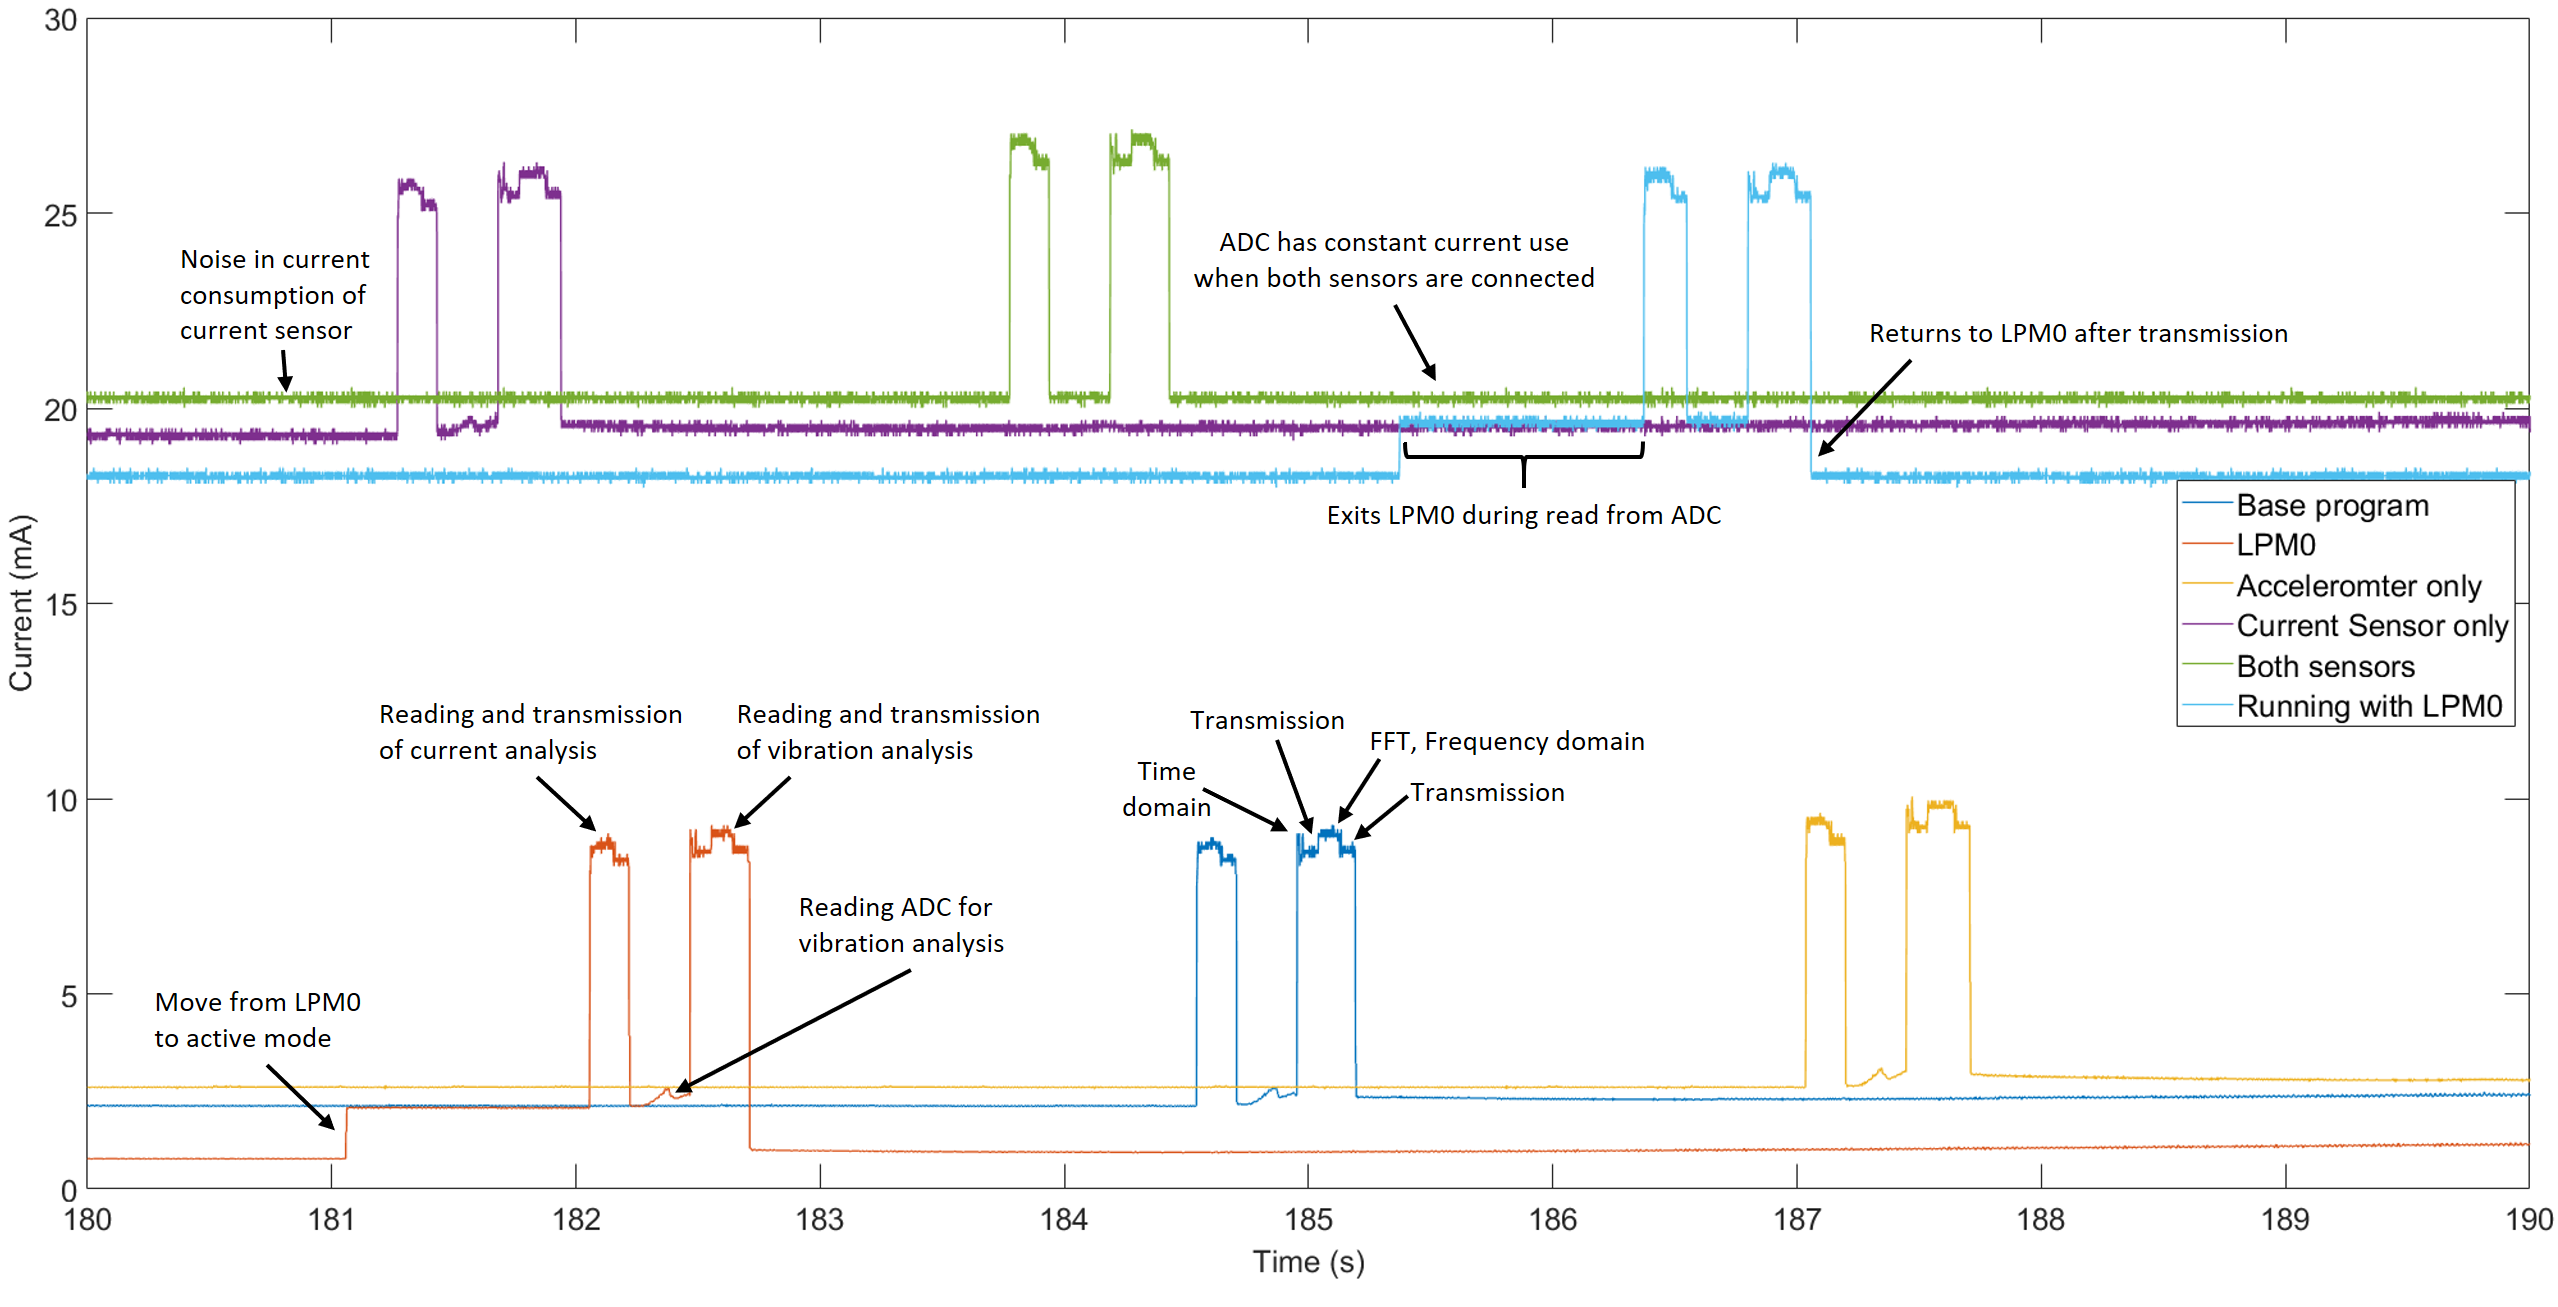
\includegraphics[width=\linewidth]{EnergyTraceNotes.png}
    \caption{Annotated current levels for different system states during reading, processing and transmission of data (signals offset in time for clarity)}
    \label{fig:EnergyTraceNotes}
\end{figure}

\begin{table}
	\begin{center}
		\begin{tabular}{lS[table-format=3.2]}%Changed c to S
			\toprule
			\textbf{Test}  & \textbf{Average Power (mW)} \\
			\midrule
            Base & 7.333\\
            LPM & 2.995\\
            Accelerometer Only \qquad & 8.902\\
            CT Only & 64.089\\
            Both Sensors & 66.980\\
            Running and LPM & 60.438\\
			\bottomrule
		\end{tabular}
		\caption{Results of power consumption tests}
		\label{tab:EnergyTrace}%Can be referenced by rest of document
	\end{center}
\end{table}